\chapter{Use cases}\label{chapter:use_cases}


% \todo{DG: Intro}

\section{Analyze blade grinder vibration}
% \todo{EB: si pu\`o dire la compagnia. Prima ci vuole una breve intro del task. E poi ci dirai quanto \`e stato difficile, etc.}
% Meglio?
In this section, we discuss how to improve an existing industrial machine, needed for blade production.
The three years old, installation has a high number of standstills (unplanned stop) with a strong impact on sales.
Furthermore, the excessive amount of vibrations on the machine has negative effect on quality of the cut, invalidating quality test results.
% I'd like to talk you about %% troppo informale
%\todo{EB: Continuare una frase cos\`i ``The full understanding of context of the problem demostrated to be crucial to...'' La frase corrente \`e troppo colloquiale}

We are also going to illustrate some difficulties encountered in vibration analysis and correlated problems, where 
the full understanding of problem's context demonstrated to be crucial.
Despite the lack of precise operational data, counter-intuitive results, the initial report was successful and helped to strengthen the methodology for further analysis.

\subsection{Initial Hypothesis}
\paragraph{Context Introduction}
\begin{figure}[ht]
    \begin{subfigure}{\textwidth}
        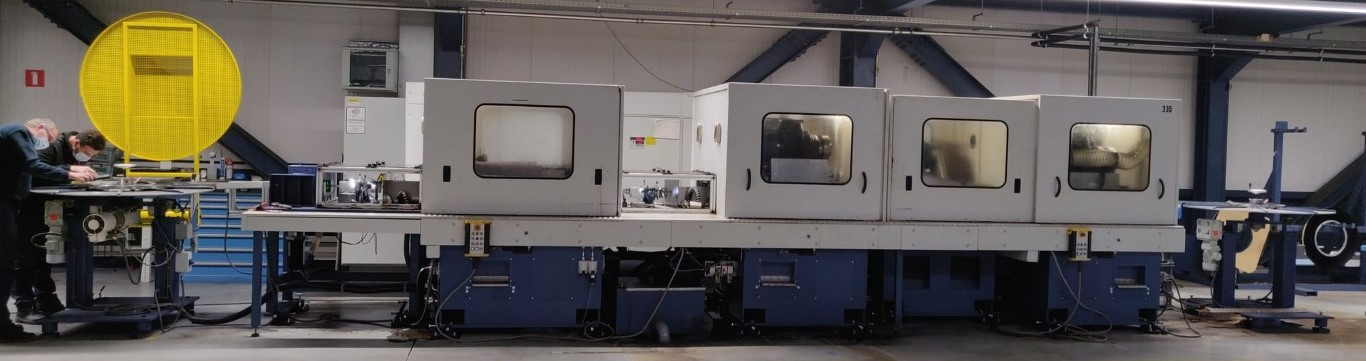
\includegraphics[width=\linewidth]{stumabo/installation/line_photo.jpg}
        \caption{Line overview: side view}
        \label{fig:line_overview}
    \end{subfigure}
    \begin{subfigure}{\textwidth}
        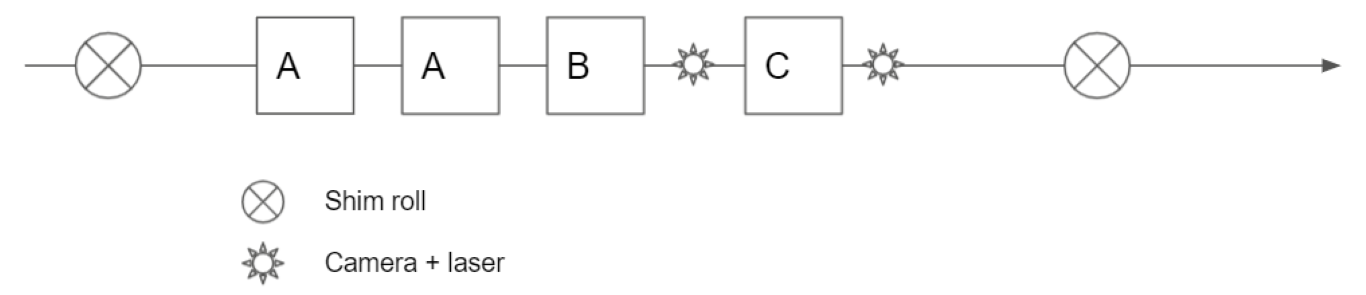
\includegraphics[width=\linewidth]{stumabo/installation/line_schematics.png}
        \caption{Line motor schematics}
        \label{fig:line_schematics}
    \end{subfigure}
    \caption{Stumabo's blade production line covered by this project}
    \label{fig:stumabo_prod_line}
\end{figure}
The subject of this monitoring operation is a blade-cutting machine line.
As shown in Figure~\ref{fig:stumabo_prod_line} there are four different stations (\subref{fig:line_overview}). Each of them has one or two motors type ${A,B,C}$ (\subref{fig:line_schematics}).
Each station has grinding stones to sharpen a blade, which is one long strip of steel passing through all the machines.
To perform their grinding task, the stones turn around their axe sharpening the steel blade, each machine in its own way.
% \todo{DG: dare definizione di campagna ad hoc? EB: questa non l'ho capita}

\paragraph{Client} Stumabo International, a manufacturer of precision blades for the food processing industry, produces several million blades per year, 
and it is known in the industry for their progressive industrial potato cutting solutions, and innovative shapes produced through hydro-cutting systems.
Stumabo also uses their knowledge to integrate the best blade in the FAM industrial mechanical cutters~\cite{Misc:stumabo_en_website}.

\subsection{Goal(s), purpose \& critical factors}
The project started in conjunction with the beginning of the internship (Oct-Nov 2021), and I had the pleasure of contributing in its early stages.
The main objective was to produce an \textit{ad-hoc}\footnote{It is usually produced only once, is more visual than a static report and, once completed, is shared with a smaller audience.} 
analysis report, that could answer specific business questions.
Unfortunately my practice ended before the second, more substantial monitoring phase of the project began, scheduled to be April 2022.
Let's see what the goals are in the long and short term and then exploring the latter.
\paragraph{Long term: project lifecycle}
\begin{itemize}
    \item[$\circledcirc$] Increase production quality through the use of continuous data analysis.
    \item[$\circledcirc$] Avoid unplanned standstill (downtime) by preventing critical component failures.
    \item[$\circledcirc$] Extends the life of machines and installation through \acl{PdM} and \acl{cm} (see Section \ref{section:maintenance})
\end{itemize}
\paragraph{Short term: \textit{ad-hoc} campaign}
\begin{itemize}
    \item[$\circledcirc$] Is  it possible to identify a strong impact of the turning of the grindstones? Perhaps a possible imbalance?
    \item[$\circledcirc$] As a general insight, do we have indication that something is causing strong vibration?
    \item[$\circledcirc$] Lastly, as preliminary path for the second stage, the \ac{CtM}, which key elements we should focus on? 
    \todo{EB: questo punto non l'ho capito, DG: meglio?}
\end{itemize}

\subsection{Project description by phases}
\begin{figure}[ht]
    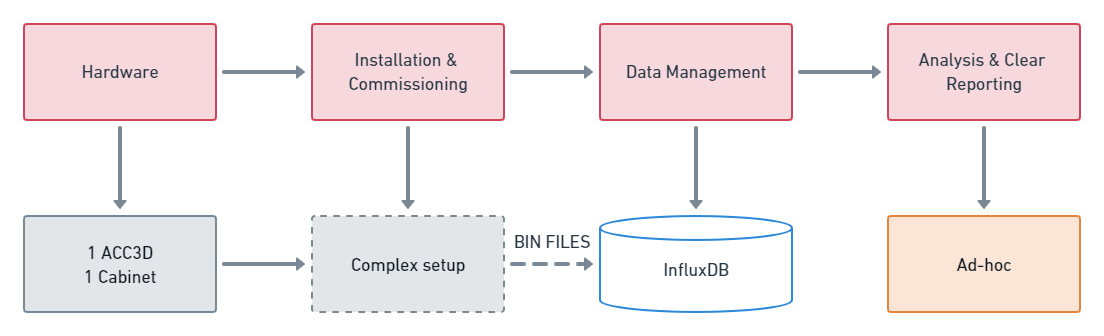
\includegraphics[width=\textwidth]{stumabo/21022_STU.png}
    \caption{Core Stages of this (full) project}
    \label{fig:stumabo_stages}
\end{figure}
As we saw earlier in Section~\ref{section:zensor_approach}, we can have two types of projects, \textit{full} and \textit{light}.
This one belongs to full or ``complete'' class, with some intense engineering (hardware \& installation) phases.  
% \todo{EB: ricordare cosa vuol dire un ``complete one' e troppo informale ``as the reader will have already guessed''.' EB: ci ho anche capito poco.}
\todo{Perch\'e less complex than big project? 
DG: perchè è una campagna di preparazione inziale.} \\
\todo{E cosa \`e un ``big'' project? big confonde, meglio full.
Magari era scrtto prima. Ma bene sia ricordarlo che aggiungere riferimento a ``prima'' DG: il riferimento era già presente ad inizio paragrafo, ne aggiungo un' altro?}

However, since this is a preparation (\textit{ad-hoc}) campaign, as mentioned earlier, it will have less complexity than a regular \textit{full} project.
To summarize it in one formula, given three variables ($f$ull, $l$ight, $s$tumabo) and ``complexity'' function $O(x)$ is true that $\forall f,l| O(l) \leq O(s) \leq O(f)$.
My contribution was to help with the analysis phase, but it's important to emphasize how the first three phases went, because they will have serious implications for data development and analysis.
\paragraph{Hardware} 
\begin{figure}[ht]
    \begin{subfigure}{0.33\textwidth}
        \centering
        
\includegraphics[height=\linewidth]{stumabo/installation/acc_station_1_blue.png}
        \caption{Installation photo}
        \label{fig:s1b_foto}
    \end{subfigure}
    \begin{subfigure}{0.33\textwidth}
        \centering
        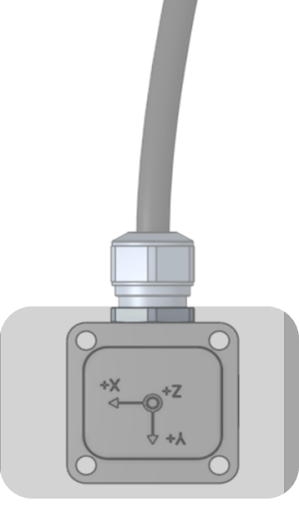
\includegraphics[height=\linewidth]{stumabo/installation/acc_render.png}
        \caption{CAD render}
        \label{fig:s1b_render}
    \end{subfigure}
    \begin{subfigure}{0.32\textwidth}
        \centering
        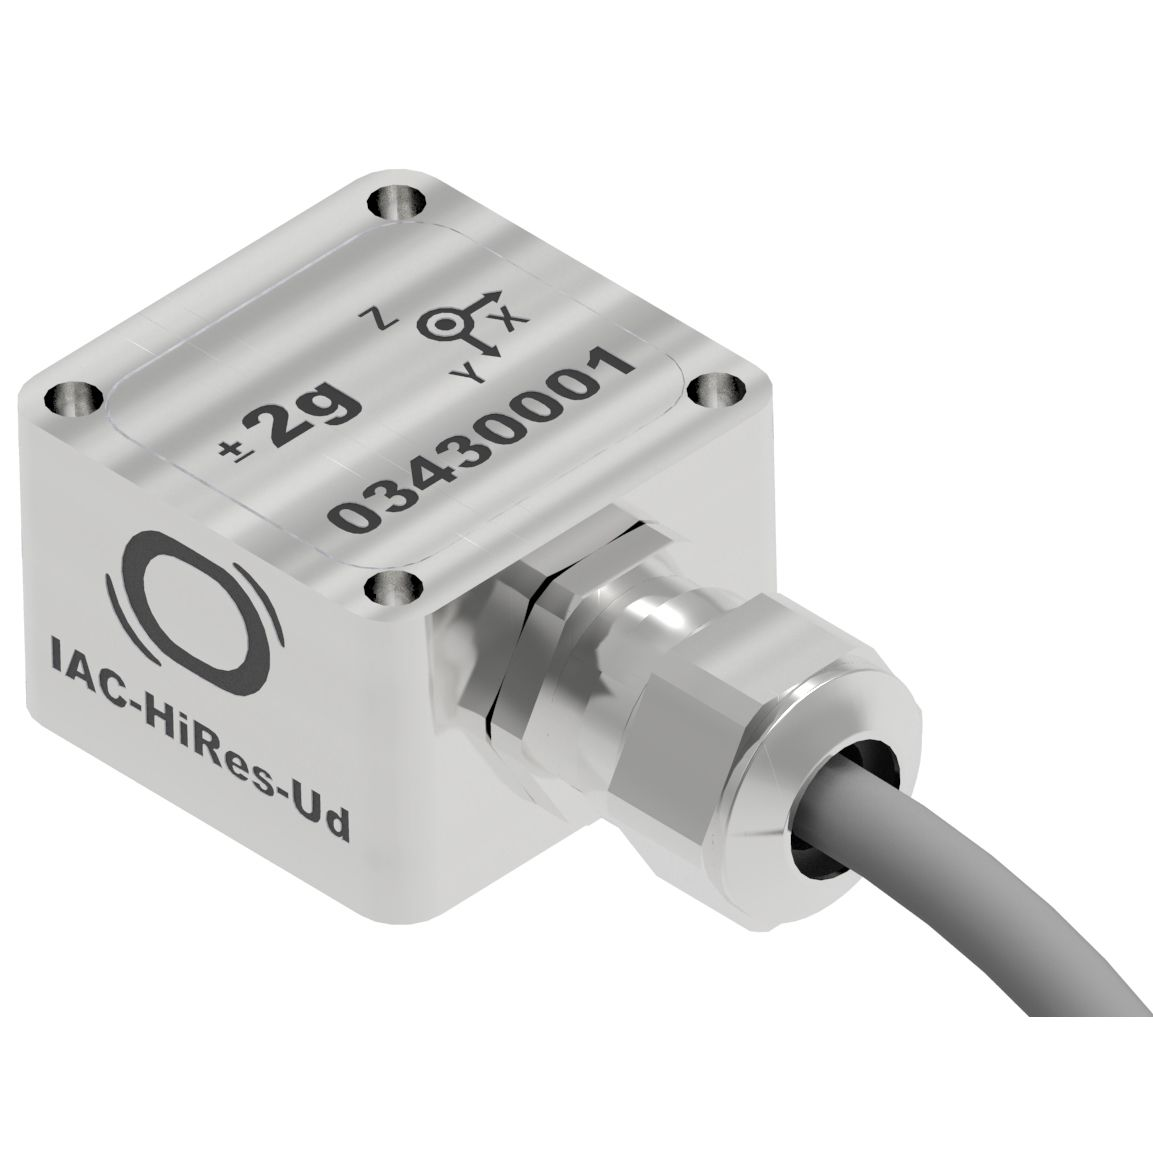
\includegraphics[height=\linewidth]{stumabo/installation/accelerometer_3_axis.jpg}
        \caption{An industrial ACC3D}
        \label{fig:stumabo_acc3d}
    \end{subfigure}
    \caption{Station 1 \textcolor{blue}{blue}: sensor setup}
    \label{fig:stu_station1_b}
\end{figure}
One 3-dimension accelerometer, called \textit{ACC3D} in Figure \ref{fig:stumabo_acc3d}, and a ``mobile cabinet'' was provided to Stumabo, 
which they placed on each of the four machine and roughly kept track of the different positions and operations in a log file.
Unfortunately, this is the only operational data available, with the following structure (see Table \ref{tab:stu_logfile}).
As it can be  seen, despite being in Flemish, it has several tags but with one big issue: start and end time are approximate and do not reflect the data trends collected by the above-mentioned sensor.
% More on that later on. \todo{EB: ``More on that later on.'' troppo informale. E forse anche grammaticalmente sbagliata}

\begin{table}[h]
    \centering
    \begin{tabularx}{\textwidth}{llllll}
        \toprule
        Datum & Start tijd & Stop tijd & Actie & Opmerkingen & Opstelling \\\midrule
        \textit{Date} & \textit{Start time} & \textit{Stop time} & \textit{Action} & \textit{Notes} & \textit{Setup} \\\midrule
        08/10/2021 & 13:19 & 13:29 & Test & Enkel \dots & grote \dots \\ % de slijpstenen van station 1 (grote snede blauwe zijde) draaien. & grote snede blauw  \\ 
        \midrule
        \dots & \dots & \dots & \dots & \dots & \dots \\\midrule
        30/11/2021 & 12:35 & 14:07 & Prod & \dots & \dots \\\bottomrule
    \end{tabularx}
    \caption{Log file structure}
    \label{tab:stu_logfile}
\end{table}

\paragraph{Installation} We must therefore clarify, before we go any further, the industrial setup: in our aid, come the engineering schematics showed in figure \ref{fig:engineering_files};
it consists in three subfigures: the first one (\subref{fig:top_view_line}) represents the same production line we saw earlier at \ref{fig:line_overview}, just from another prospective. 
This view from above makes it easier for us to identify some important elements, e.g.\ how many stones are present for each station.
It is essential to clarify a simple convention: within Stumabo the right side of the line is referred to as \textcolor{red}{red}, \textit{rood} in Flemish, and, in the same way, 
the left side will be referred to as \textcolor{blue}{blue}, \textit{blauw}. 
Speaking about colors, we can now make a direct connection with Figure (\subref{fig:blade_evolution}), which shows us the evolution of the blade during the process.
% Considering that grinding stones turn around their axe sharpening the steel blade.
First it is sharpened, from the 1st \textcolor{blue}{blue} station, on the left side, and then it passes to the 1st \textcolor{red}{red} station, where it will be rolled on the right side. 
Same goes for 2nd and 3rd station, that have two grinders aligned. 

Now that we are aware of how the industrial process works, let's move on to diagram (\subref{fig:local_to_global}).
It represents in more detail how the sensor has been installed and what consequences it has with respect to the coordinate system, 
a somewhat complex issue that has caused several doubts and discussions in the analysis phase. This would therefore appear to be a good point to take stock of the situation.
The accelerometer was installed within the line, adjacent to the stones and close to the blade, by means of a round magnet, as shown in Figure \ref{fig:s1b_foto}.
Moreover, the same device was placed, at different times in different stations, mirrored on both sides, except the last one, for a total of five different locations: 
${S_{1}\textcolor{red}{R}\&\textcolor{blue}{B}, S_{2}\textcolor{red}{R}\&\textcolor{blue}{B}, S_{3}\textcolor{blue}{B}}$ as shown in the bottom part of Figure \ref{fig:top_view_line}.

It follows that \textbf{two} different \textbf{reference systems} are present:
\begin{itemize}\label{item:double_system}
    \item local $(x,y,z)$ for each sensor placement;
    \item global $(X,Y,Z)$ for the entire production line.
\end{itemize}
We can see some refences of this important aspect in the mentioned figures alongside. % here on the side 
This dual model well abstracts the reality, but does not allow a comparison between the various stations, which instead we would like to carry out to achieve the initial goals.
So it will be necessary to transform everything in global coordinates, taking into account two additional factors:
 \textit{sensor orientation} and 
 \textit{installation angle}. 
\begin{figure}[!htp]
    \begin{subfigure}{\textwidth}
        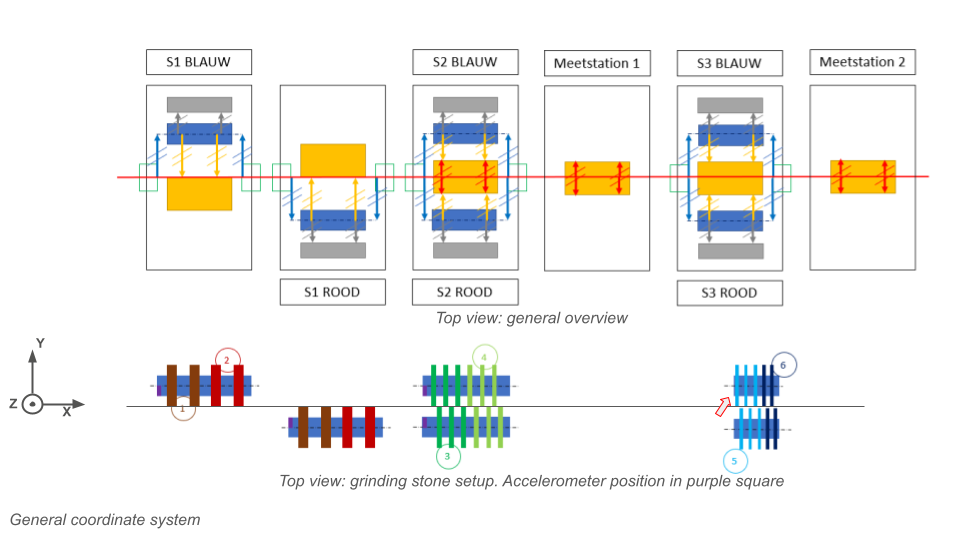
\includegraphics[width=.95\linewidth]{stumabo/installation/general_cordinate_system.png}
        \caption{Top view overview of stations plus grinding stones detail.
            Purple dots on the bottom details are where the $3D$ accelerometer was placed}
        \label{fig:top_view_line}
    \end{subfigure}
    \begin{subfigure}{\textwidth}
        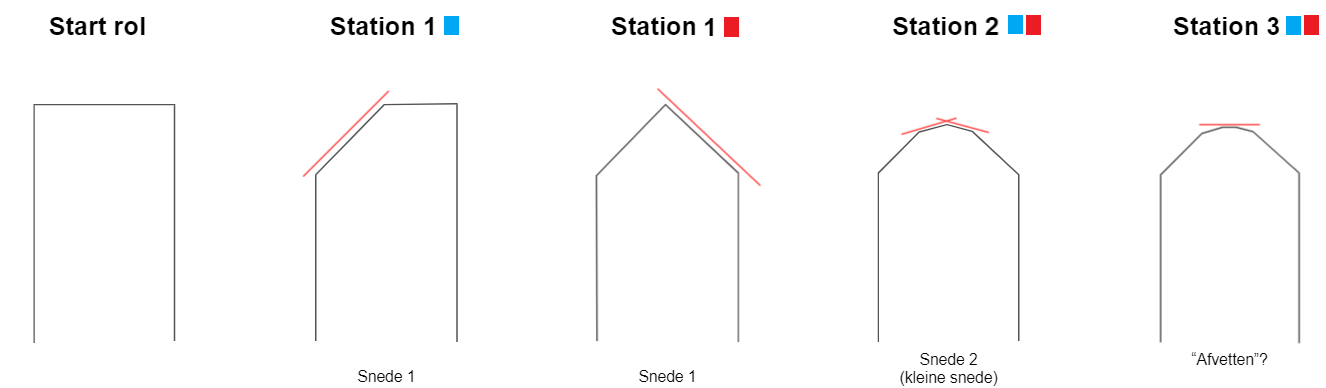
\includegraphics[width=.95\linewidth]{stumabo/installation/blade_processing.png}
        \caption{Blade evolution, a sketched overview of the cut by station}
        \label{fig:blade_evolution}
    \end{subfigure}
    \begin{subfigure}{\textwidth}
        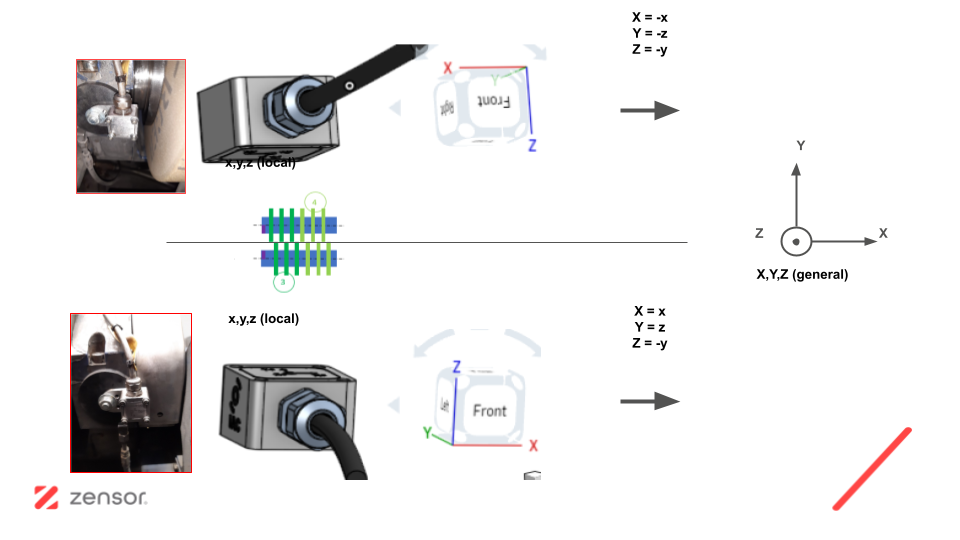
\includegraphics[width=.95\linewidth]{stumabo/installation/local_to_global.png}
        \caption{From local to general coordinate system, top view}
        \label{fig:local_to_global}
    \end{subfigure}
    \caption{Engineering schematic are also important during analysis}
    \label{fig:engineering_files}
\end{figure}

\begin{itemize}
    \item \textbf{Sensor Orientation}: 
    going back on Figure \ref{fig:stu_station1_b}, we can see how the sensor has been installed horizontally, with the $x$-axis as parallel as possible to the blade ($X$) with 
    the help of a level. \todo{EB: check English: ``tolerates''? DG: esiste ed è usato}
    This tolerating some errors due to disturbing factors such as color, dirt and imperfections of the metal.
    Furthermore, the latter is installed upside down, i.e.\ parallel to the $Z$ axis as shown in the Render \ref{fig:s1b_render}.
    \item \textbf{Installation Angle}:
    We had to take also into account that the machines have various angles to the ideal $Z$-axis, this was measured on site and varies from station to station, from 5° to 12° degrees.
\end{itemize}
We will delve into both aspects in the final stage of analysis, but now we would like to clarify following equation-mapping (\ref{eq:op}) from \textit{local} to \textit{global} coordinate.
Here $\widehat{widehat}$ stands for the \textit{rotation} operator and $\underline{underline}$ for \textit{transposition}. 
\begin{equation}
    \left\{ \begin{array}{cl}
        x = \alpha & \Rightarrow  \ x = \widehat{\alpha} \ \Rightarrow  \ X = \underline{\widehat{\alpha}} \\
        y = \beta & \Rightarrow  \ y = \widehat{\beta} \ \Rightarrow  \ Y = \underline{\widehat{\beta}} \\ 
        z = \gamma & \Rightarrow  \ z = \widehat{\gamma} \ \Rightarrow  \ Z = \underline{\widehat{\gamma}}
        \end{array} \right.
    \label{eq:op}
\end{equation}
We now move on to the following phase.

\paragraph{Data Management}
As stated previously a single sensor was placed in different locations, remaining on for the duration of the ad hoc project. We will therefore have a single data stream.
The data flow is as follows: from the sensor to the cabinet to AWS and, finally, InfluxDB.
\begin{figure}[ht]
    % Mettere più grandi?
    \begin{subfigure}{.495\textwidth}
        \includegraphics[width=\textwidth]{stumabo/analysis/60Hz-raw-vibration.pdf}
        \caption{\texttt{60Hz} raw vibration}
        \label{fig:stu_60Hz_raw}
    \end{subfigure}
    \begin{subfigure}{.495\textwidth}
        \includegraphics[width=\textwidth]{stumabo/analysis/1Hz-raw-vibration.pdf}
        \caption{\texttt{1Hz} raw vibration}
        \label{fig:stu_1Hz_raw}
    \end{subfigure}
    \caption{\acl{EDA} on 1° block, station 1 \textcolor{blue}{blue}}
    \label{fig:stu_2_raw_data}
\end{figure}

\todo{EB: mi pare che $x$, $y$, $z$ vengano utilizati a volte minuscoli, altre maiuscoli. C'\`e un motivo? Spiegare motivo, oppure, se non c'\`e uniformare notazione} \\
\todo{DG: il paragrafo precedente (installation) è dedicato principalmente a questa tematica ...}
% \todo{EB: gli Hertz normalmente si abbreviano con ``Hz'' non ``Hz''} 
As a reminder: lowercase stands for local frame of reference, while upper is for global as explained before at \ref{item:double_system}.

I would like to point out that, at cabinet level, two separate binary files are created, where $x$ and $z$ channels are stored together and, instead $y$ channel is kept separated. 
Moreover, for each sensor channel, all vibrations are recorded at \texttt{60Hz}, or 60 points per second, for a total of 180 per second (\ref{sub@fig:stu_60Hz_raw}).
As you can easily imagine when you want to visualize, e.g.\ doing some \ac{EDA} as discussed in subsection \ref{subsubsec:eda}, 
and investigate hours and hours of data these are way too many data points.
This is the reason why Lambda\footnote{AWS Lambda is an event-driven, serverless computing platform \url{https://aws.amazon.com/it/lambda/}}, 
during data ingestion, aggregates the data using the mean function, and reduces the frequency to \texttt{1Hz} (\ref{sub@fig:stu_1Hz_raw}), i.e.\ 
performs a down sampling operation. It then saves both streams in the \ac{tsdb} as separate measurements as shown in Figure \ref{fig:stu_aly_overview}. 
It is an important element that will be useful later in analysis phase.

\begin{figure}[ht]
    \begin{subfigure}{.495\textwidth}
        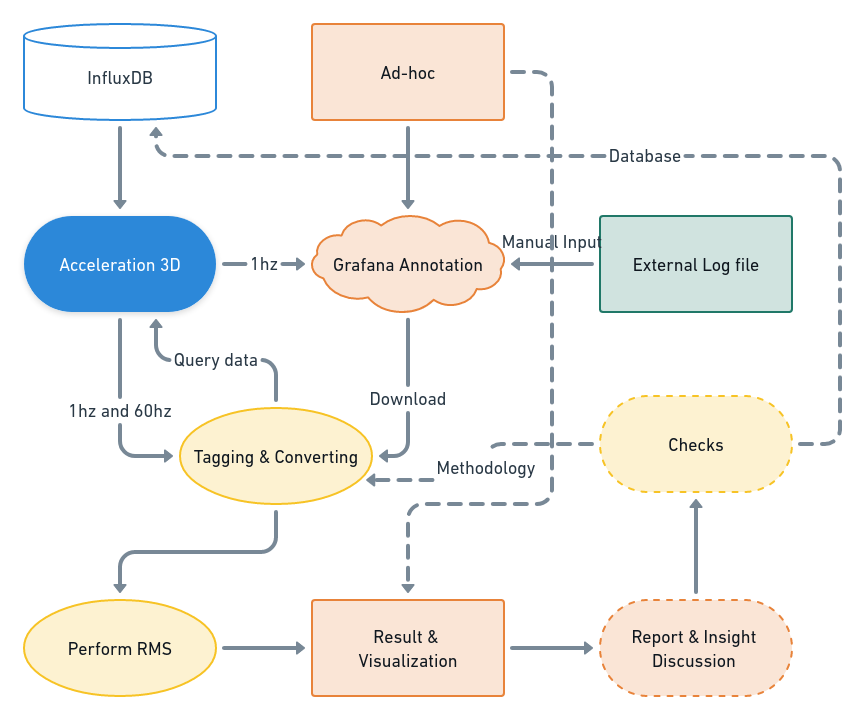
\includegraphics[width=\linewidth]{stumabo/analysis/analysis_flow.png}
        \caption{Data Management and Analysis overview}
        \label{fig:stu_aly_overview}
    \end{subfigure}
    \begin{subfigure}{.495\textwidth}
        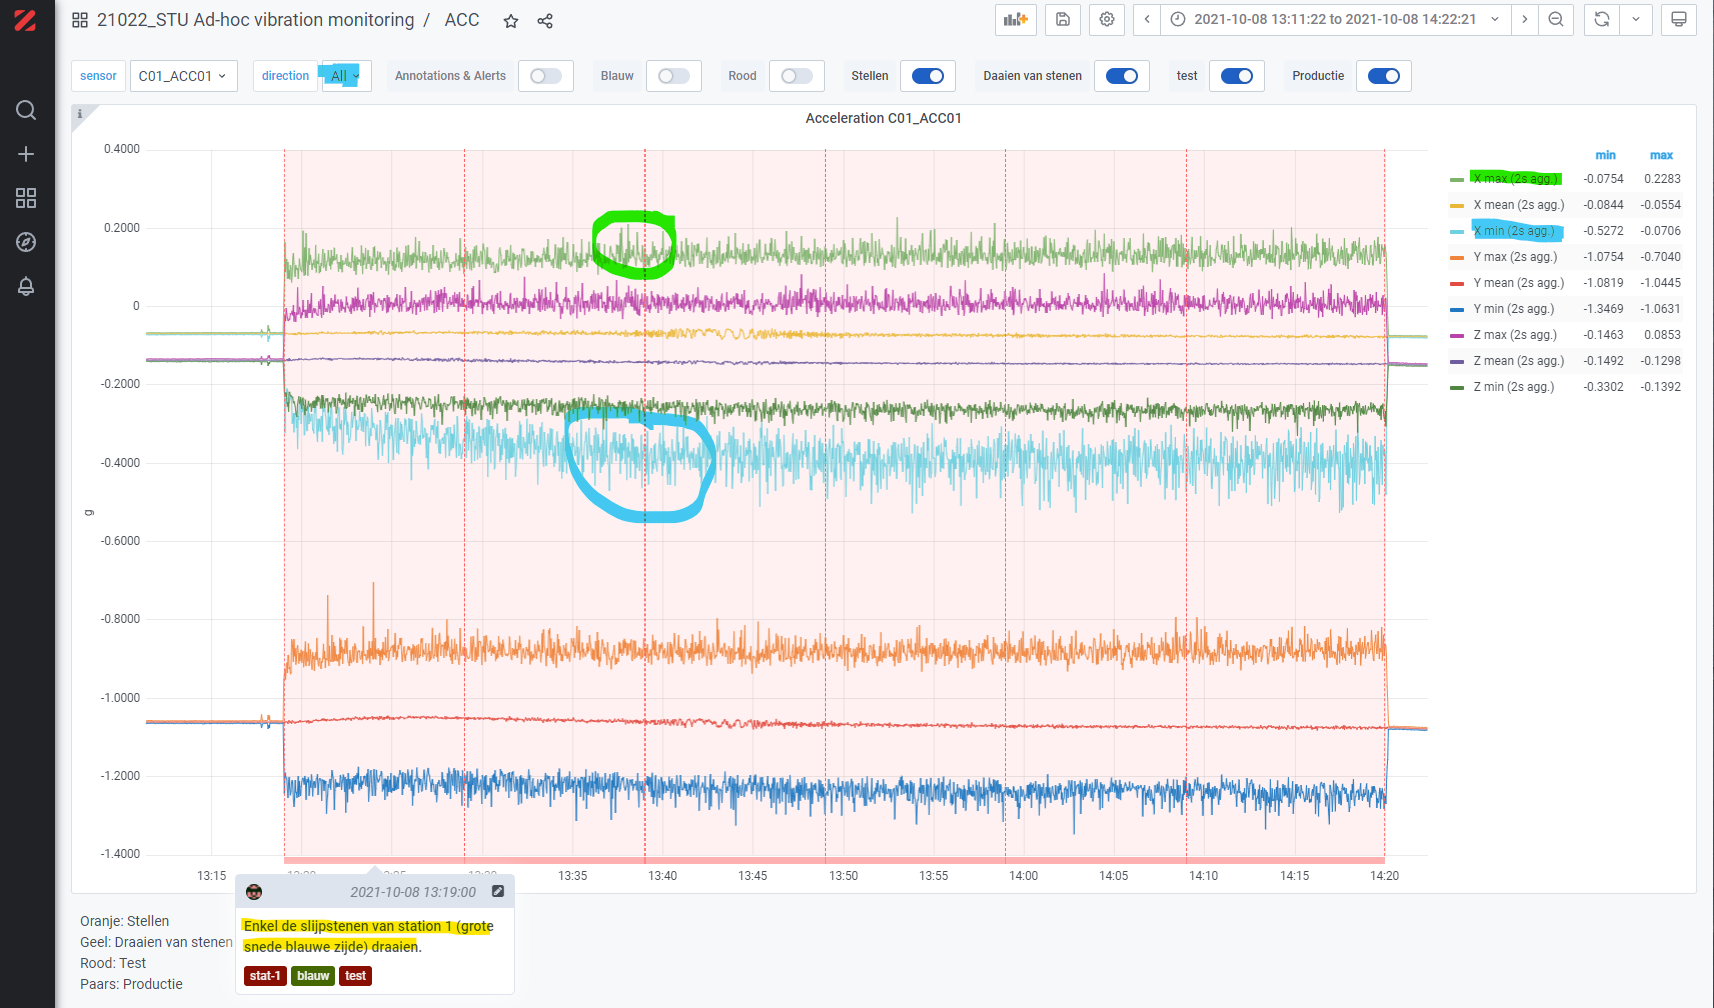
\includegraphics[width=\linewidth, height=4.6cm]{stumabo/analysis/grafana-annotation.png} 
        \caption{Annotation process}
        \label{fig:stu_annotation}
    \end{subfigure}
    % \caption{}
    % \label{fig:stu_2_aly}
\end{figure}

\paragraph{Analysis}
This is where most of my work and time went, my first task was to perform some \acl{EDA} over the \texttt{acc\_1Hz} measurement using Grafana (\ref{sub@fig:stu_aly_overview}).
Since the cabinet was never turned off while sending data for approximately two months, except for five days, between 13/10 and 18/10, it was clear from the start that most of 
the signal was useless, ``flat'' stationary data with no movement e.g.\ during night hours when the servo motors were off. 
Another big problem was that there was no distinction whatsoever between different sensor installation positions.
To solve these and other smaller issues a preliminary data labeling step was performed directly on the visualization tool, using the Excel log file as source of 
operational data, with all the limitations involved. The task was performed in-place using the Annotation UI, dividing the measurement in smaller blocks of variable length 
as demonstrated in Figure \ref{fig:stu_annotation}. While being tedious, it was strictly necessary, otherwise no meaningful analysis could have been performed.

% \todo{EB: troppo informale: Let's go through the procedure together. }
% \todo{DG: non saprei come sostiturlo, quindi rimuovo}

The idea is to isolate relevant data, in other terms data that is available, and we know what it represents keeping in mind we are interested in finding sub zones 
where data seems to be not varying (so much): for instance we would like to exclude the acceleration and deceleration phases of servo motors.
For each client log entry, we create an equivalent annotation entry, with the caveat that there could be more than one behavior block identified per run, so we have two unique identifiers, a Block ID and a Run ID. 
Each block will have several variables like operation \{TEST, PROD, \dots \}, color \{\textcolor{blue}{Blue} and \textcolor{red}{Red}\}, station $\{1,2,3\}$, and so on. 
These variables will be our tags columns $\{n+1, n+2, n+3, \dots\, k\}$ in our final result Table C. To give an approximate order of magnitude, about 110 annotations, hence blocks, were made.
The next step was to download the annotations, using Grafana's REST API, and to transition to a better data structure: from intermediate JSON to structured DataFrame.
Once this metadata was in place, we could proceed with the more complex section of the analytics.
Once again our main concern was to study the amplitude of vibration. So for each \emph{annotated block} we: 
\begin{enumerate}
    \item retrieved ACC data through iterative queries to InfluxDB, using start and end time;
    \item manipulated it, using vector calculus, for performing rotation and translation operations;
    \item returned the \ac{RMS} values for each individual axes $X,Y,Z$;
\end{enumerate}
We are now going to take a closer look at the various operations: % troppo informale? EB: si DG:meglio?
as far as the first one is concerned, nothing too complicated, thanks to zensor library we can easily retrieve our time series data in a shape of a pandas DataFrame.
For the second point, here now we do not dwell too much technical details, it was agreed to combine the two operations into one (see Equation \ref{eq:op}).
So what we end up doing was performing dot product among vector $u$ and matrix $R_X(\phi)$, in formula: $R_X(\phi)u = u$.
With no signs assigned to the angles, that we know from engineering files, the basic translation $+$ rotation matrix on $X$-axis $R_X(\phi)$ is:
\begin{itemize}
    \item \textcolor{blue}{Blue}: \( \left\{ 
        \begin{array}{cl} 
            Y & = \ -y sin(\phi) + z cos(\phi) \\
            Z & = \ -y cos(\phi) - z sin(\phi) 
        \end{array} \right. 
        \Rightarrow  
        \begin{bmatrix}
            1 & 0 & 0 \\
            0 & -sin(\phi) & cos(\phi)  \\
            0 & -cos(\phi) & -sin(\phi)  
        \end{bmatrix} \)
    \item \textcolor{red}{Red}: \( \left\{ 
        \begin{array}{cl}
            Y & = \ y sin(\phi) - z cos(\phi) \\
            Z & = \ -y cos(\phi) + z sin(\phi) 
        \end{array} \right. 
        \Rightarrow
        \begin{bmatrix}
            1 & 0 & 0 \\
            0 & sin(\phi) & -cos(\phi)  \\
            0 & -cos(\phi) & sin(\phi)  
        \end{bmatrix} \)
\end{itemize}
Lastly for the third step is important to point out that, for each direction, before the RMS is calculated, the average of the time-block is determined. 
This average will be subtracted from the array values, as to only monitor the RMS of the relative acceleration.

These three operation were combined in one python function and used alongside Pandas internals. So the methodology was firstly ``called'' on \texttt{1Hz} data for testing the procedure, that took approximately $15$ minutes of CPU time, 
and then on the higher frequency data, \texttt{60Hz} where instead took more than $4$ hours. At Figure \ref{fig:stu_3_rms} we observe three plots.
For all of them we have common elements. The x-axis label is our block identifier (Block ID), while on the y-axis represent the overall RMS value of the block itself. 
It is quite evident how the two graphs represent similar signals but of different order of magnitude. In case \ref{sub@fig:stu_1Hz_rms} we have a $[min, max]$ range of $[0,20] * 10^{-4}$ 
while in \ref{sub@fig:stu_60Hz_rms} is $[0,25] * 10^{-2}$ which makes direct comparison difficult, see Plot \ref{sub@fig:stu_1_vs_60}.
In particular, the \texttt{60Hz} trend seems to be more constant and gradual, while \texttt{1Hz} is characterized by strong peaks. It is clear that station 2 cause most of the vibration, 
as we would expect, by his design with two engines closer to each other.

\begin{figure}[htp]
    \begin{subfigure}{.495\textwidth}
        \includegraphics[width=\textwidth]{stumabo/analysis/1Hz-ad-hoc.pdf}
        \caption{\texttt{1Hz} RMS values}
        \label{fig:stu_1Hz_rms}
    \end{subfigure}
    \begin{subfigure}{.495\textwidth}
        \includegraphics[width=\textwidth]{stumabo/analysis/60Hz-ad-hoc.pdf}
        \caption{\texttt{60Hz} RMS values}
        \label{fig:stu_60Hz_rms}
    \end{subfigure}
    \begin{subfigure}{\textwidth}
        \includegraphics[width=\textwidth]{stumabo/analysis/1Hz-vs-60Hz.pdf}
        \caption{\texttt{1Hz} and \texttt{60Hz} RMS values}
        \label{fig:stu_1_vs_60}
    \end{subfigure}
    \caption{RMS amplitude comparison between low and high frequency data}
    \label{fig:stu_3_rms}
\end{figure}

After all of these operations, we combined \texttt{1Hz} numerical values to the previously prepared metadata to achieve an interesting intermediate result that has approximately this aspect. 
% \todo{EB: ``intermediate'' ==> ``intermediate''?}
Run ID and Block ID were removed here for relevance purposes (see Table \ref{tab:stu_intermediate_res}).  
These results were then discussed and checked with a more experienced colleague, who had more domain knowledge. 
He also continued with the analysis, comparing, for example, different stations for the same type of operation. 
I decided not to discuss his insights, here in this report, as they are not the result of my work but a more direct consequence.
% TEST    = Test   
% DASTE   = Draaien van stenen   
% STEL    = Stellen   
% PROD    = Productie 
\begin{table}[ht]
    \centering
    \begin{tabularx}{\textwidth}{@{}lllllllll@{}}
    \toprule
    start & einde & actie & kant & stat & draaien & $X$ & $Y$ & $Z$ \\ \midrule
    13:19:01 & 13:29:01 & TEST & \textcolor{blue}{B} & 1 & 1 & 131 & 176 & 592 \\ 
    13:29:01 & 13:39:00 & TEST & \textcolor{blue}{B} & 1 & 1,2 & 160 & 143 & 461 \\  
    13:38:58 & 13:49:01 & TEST & \textcolor{blue}{B} & 1 & 1,2,3\textcolor{blue}{B} & 132 & 166 & 356 \\ 
    13:48:59 & 13:59:00 & TEST & \textcolor{blue}{B} & 1 & 1,2,3\textcolor{red}{R} & 113 & 149 & 244  \\
    13:59:00 & 14:08:59 & TEST & \textcolor{blue}{B} & 1 & 1,2,3\textcolor{blue}{B},3\textcolor{red}{R} & 145 & 143 & 217 \\ 
    14:09:00 & 14:20:00 & TEST & \textcolor{blue}{B} & 1 & 1,2,3\textcolor{blue}{B},3\textcolor{red}{R},4 & 176 & 153 & 294 \\ 
    \dots \\
    10:04:00 & 12:35:00 & DASTE & \textcolor{blue}{B} & 3 & 1,2,3\textcolor{blue}{B},3\textcolor{red}{R},4 & 630 & 542 & 1489 \\
    \bottomrule
    \end{tabularx}
    \caption{intermediate result: numerical RMS \texttt{1Hz} values are given using engineering notation: $10^{-6}$}
    \label{tab:stu_intermediate_res}
\end{table}

\subsection{Conclusion}
Stumabo ad-hoc analysis showed, overall, insightful findings. For instance station 1 \textcolor{blue}{blue} has higher vibration than it should, 
and it will be further investigated with spectral analysis for better identify the root cause.
There was a less intuitive result though: vibration amplitudes (RMS) in $X$ direction, along the blade going through the grinding stone stations,
seemed more prominent than in $Y$ direction, also horizontal but perpendicular to the blade direction.
Before digging deeper into this, we wanted to check on our side if these axes can't have been switched somewhere.

The machines (motor, stones \dots) and stones turning both causes vibrations. As discussed previously, for keeping temperatures low, cooling fluid is sometimes applied to the stones, 
where it is absorbed. When drying, we noticed higher vibrations as the liquid isn't all over the stone anymore, but going to the outside gradually.
Anyway, the turning would intuitively cause more vibrations perpendicular to their rotating axe ($Y$) and ($Z$), not along their axe ($X$), 
but in the analysis we saw relatively higher vibrations along the blade axe ($X$) than perpendicular to it ($Y$), even though ($Z$), vertically, is still highest. 
After successfully double-checking back-end, Lambda configuration and the \ac{PLC} programming, we couldn't confirm 100\% the cabling connection, but with a small margin of 
error, we can confirm that, indeed, $X$ and $Y$ are \textbf{not} switched. Further analysis will eventually debunk that. 


% Main concern: amplitude of vibration
% Run ID, Block ID {0,1,...,n}: for each client log entry – there could be more than one behaviour BLOCK identified per RUN
% Actie (4 tags)
%         TEST     = Test   
%         DASTE = Draaien van stenen   
%         STEL    = Stellen   
%        PROD     = Productie    
% Kant
% Station {0,1,...,4}
% Color 
% {blauw, rood}
% Coolant {true, false}
% \begin{figure}[ht]
%     \includegraphics[width=\textwidth]{stumabo/analysis/1Hz-vs-60Hz.pdf}
%     \caption{\texttt{1Hz} and \texttt{60Hz} RMS values}
%     \label{fig:stu_1_vs_60}
% \end{figure}
% A potential deeper investigation for the ad-hoc data is being proposed as of February 2022

% \section{Climbing the information Ladder and difference between data and information}
% General note: I wouldn't go into too much detail. but I would tend to focus more on where I contributed to the success of the project, for better or worse.

% \section{Monitor electricity consumption}

% \textit{MOBI Hospital} -
% \textit{Student Dorms} -
% \textit{V U B Etterbeek Campus} -

% One possible idea would be to compare the three different projects \textbf{20012/20013/21025} and highlight the commonalities, e.g. the purpose, the fact that they have the 'same' client [although I think they are different research groups], and the differences, such as the data collection and the target user of the dashboards or project age etc.

% \paragraph{Vrije Universiteit Brussel}
% The Vrije Universiteit Brussel is a Dutch and English-speaking research university located in Brussels, Belgium. Motto: \textit{"Conquering darkness by science"}


% \section{Increase efficiency of tomato company}
% \textbf{21024}: Finally, I'd like to tell the tale of \cite{Misc:stoffels_en_website}:
% \begin{itemize}
%     \item how the demo of this project was launched with an intense daily sprint, followed by a duo collaboration with another inter (Kasia);
%     \item how this project is a bit of a white fly compared to the zensor-standard project;
%     \item  was also an opportunity for me to test my skills in the role of backend rather than analysis.
% \end{itemize}
